%beamer

% Comment/uncomment this line to toggle handout mode
\newcommand{\handout}{}

%% Beamer-Klasse im korrekten Modus
\ifdefined \handout
\documentclass[handout]{beamer} % Handout mode
\else
\documentclass{beamer}
\fi

%% UTF-8-Encoding
\usepackage[utf8]{inputenc}

\input{../framework/gbi-macros}
\usepackage[blue]{../framework/thwregex}
\usepackage{environ}
\usepackage{bm}
\usepackage{calc}
\usepackage{varwidth}
\usepackage{wasysym}
\usepackage{mathtools}


% Das ist der KIT-Stil
%\usepackage{../TutTexbib/beamerthemekit}
\usepackage[deutsch,titlepage0]{../framework/KIT/beamerthemeKITmod}
\TitleImage[width=\titleimagewd]{../figures/titlepage.jpg}
%\usetheme[deutsch,titlepage0]{KIT}

% Include PDFs
\usepackage{pdfpages}

% Libertine font (Original GBI font)
\usepackage{libertine}
%\renewcommand*\familydefault{\sfdefault}  %% Only if the base font of the document is to be sans serif

% Nicer math symbols
\usepackage{eulervm}
%\usepackage{mathpazo}
\renewcommand\ttdefault{cmtt} % Computer Modern typewriter font, see lecture slides.

\usepackage{csquotes}

%%%%%%

%% Schönere Schriften
\usepackage[TS1,T1]{fontenc}

%% Bibliothek für Graphiken
\usepackage{graphicx}

%% der wird sowieso in jeder Datei gesetzt
\graphicspath{{../figures/}}

%% Anzeigetiefe für Inhaltsverzeichnis: 1 Stufe
\setcounter{tocdepth}{1}

%% Hyperlinks
\usepackage{hyperref}
% I don't know why, but this works and only includes sections and NOT subsections in the pdf-bookmarks.
\hypersetup{bookmarksdepth=subsection} 

%\usepackage{lmodern}
\usepackage{colortbl}
\usepackage[absolute,overlay]{textpos}
\usepackage{listings}
\usepackage{forloop}
%\usepackage{algorithmic} % PseudoCode package 

\usepackage{tikz}
\usetikzlibrary{matrix}
\usetikzlibrary{arrows.meta}
\usetikzlibrary{automata}
\usetikzlibrary{tikzmark}
\usetikzlibrary{positioning}

% Why has no-one come up with this yet? I mean, seriously. -.-
\tikzstyle{loop below right} = [loop, out=-60,in=-30, looseness=7]
\tikzstyle{loop below left} = [loop, out=-150,in=-120, looseness=7]
\tikzstyle{loop above right} = [loop, out=60,in=30, looseness=7]
\tikzstyle{loop above left} = [loop, out=150,in=120, looseness=7]
\tikzstyle{loop right below} = [loop below right]
\tikzstyle{loop left below} = [loop below left]
\tikzstyle{loop right above} = [loop above right]
\tikzstyle{loop left above} = [loop above left]

% Needed for gbi-macros
\usepackage{xspace}

%%%%%%

%% Verbatim
\usepackage{moreverb}

%%%%%%%%%%%%%%%%%%%%%%%%%%%%%%%%%%%% Copy end

%% Tabellen
\usepackage{array}
\usepackage{multicol}
\usepackage{hhline}

%% Bibliotheken für viele mathematische Symbole
\usepackage{amsmath, amsfonts, amssymb}

%% Deutsche Silbentrennung und Beschriftungen
\usepackage[ngerman]{babel}

\usepackage{kbordermatrix}

% kbordermatrix settings
\renewcommand{\kbldelim}{(} % Left delimiter
\renewcommand{\kbrdelim}{)} % Right delimiter

\input{../config.tex}



% define custom \handout command flag if handout mode is toggled  #DirtyAsHellButWell...
\only<beamer:0>{\def\handout{}} %beamer:0 == handout mode

\newcommand{\R}{\mathbb{R}}
\newcommand{\N}{\mathbb{N}}
\newcommand{\Z}{\mathbb{Z}}
\newcommand{\Q}{\mathbb{Q}}
\newcommand{\BB}{\mathbb{B}}
\newcommand{\C}{\mathbb{C}}
\newcommand{\K}{\mathbb{K}}
\newcommand{\G}{\mathbb{G}}
\newcommand{\nullel}{\mathcal{O}}
\newcommand{\einsel}{\mathds{1}}
\newcommand{\Pot}{\mathcal{P}}
\renewcommand{\O}{\text{O}}

\def\word#1{\hbox{\textcolor{blue}{\texttt{#1}}}}
\let\literal\word
\def\mword#1{\hbox{\textcolor{blue}{$\mathtt{#1}$}}}  % math word
\def\sp{\scalebox{1}[.5]{\textvisiblespace}}
\def\wordsp{\word{\sp}}

%\newcommand{\literal}[1]{\textcolor{blue}{\texttt{#1}}}
\newcommand{\realTilde}{\textasciitilde \ }
\newcommand{\setsize}[1]{\ensuremath{\left\lvert #1 \right\rvert}}
\newcommand{\size}[1]{\setsize{#1}}  % Shame on you, TeXStudio...
\newcommand{\set}[1]{\left\{#1\right\}}
\newcommand{\tuple}[1]{\left(#1\right)}
\newcommand{\normalvar}[1]{\text{$#1$}}

% Modified by DJ
\let\oldemptyset\emptyset
\let\emptyset\varnothing % proper emptyset

\newcommand{\boder}{\ensuremath{\mathbin{\textcolor{blue}{\vee}}}\xspace}
\newcommand{\bund}{\ensuremath{\mathbin{\textcolor{blue}{\wedge}}}\xspace}
\newcommand{\bimp}{\ensuremath{\mathrel{\textcolor{blue}{\to}}}\xspace}
\newcommand{\bgdw}{\ensuremath{\mathrel{\textcolor{blue}{\leftrightarrow}}}\xspace}
\newcommand{\bnot}{\ensuremath{\textcolor{blue}{\neg}}\xspace}
\newcommand{\bone}{\ensuremath{\textcolor{blue}{1}}\text{}}
\newcommand{\bzero}{\ensuremath{\textcolor{blue}{0}}\text{}}
\newcommand{\bleftBr}{\ensuremath{\textcolor{blue}{\texttt{(}}}\text{}}
\newcommand{\brightBr}{\ensuremath{\textcolor{blue}{\texttt{)}}}\text{}}

% Fix of \b... commands:

\renewcommand{\boder}{\alor}
\renewcommand{\bund}{\aland}
\renewcommand{\bimp}{\alimpl}
\renewcommand{\bgdw}{\aleqv}
\renewcommand{\bnot}{\alnot}
\renewcommand{\bleftBr}{\alka}
\renewcommand{\brightBr}{\alkz}
\newcommand{\alA}{\word A}
\newcommand{\alB}{\word B}
\newcommand{\alC}{\word C}

\newcommand{\plB}{\plfoo{B}}
\newcommand{\plE}{\plfoo{E}}

\newcommand{\summe}[2]{\sum\limits_{#1}^{#2}}
\newcommand{\limes}[1]{\lim\limits_{#1}}

%\newcommand{\numpp}{\advance \value{weeknum} by -2 \theweeknum \advance \value{weeknum} by 2}
%\newcommand{\nump}{\advance \value{weeknum} by -1 \theweeknum \advance \value{weeknum} by 1}

\newcommand{\mycomment}[1]{}
\newcommand{\Comment}[1]{}

%% DISCLAIMER START 
% It is INSANELY IMPORTANT NOT TO DO THIS OUTSIDE BEAMER CLASS! IN ARTCILE DOCUMENTS, THIS IS VERY LIKELY TO BUG AROUND!
\makeatletter%
\@ifclassloaded{beamer}%
{
	% TODO 
	% no time... later.   (= never -.-)
	% redefine section to ignore multiple \section calls with the same title
}%
{
	\errmessage{ERROR: section command redefinition outside of beamer class document! Please contact the author of this code or read the F-ing disclaimer.}
}%
\makeatother%
%% DISCLAIMER END

\newcounter{abc}
\newenvironment{alist}{
  \begin{list}{(\alph{abc})}{
      \usecounter{abc}\setlength{\leftmargin}{8mm}\setlength{\labelsep}{2mm}
    }
}{\end{list}}


\newcommand{\stdarraystretch}{1.20}
\renewcommand{\arraystretch}{\stdarraystretch}  % for proper row spacing in tables

\newcommand{\morescalingdelimiters}{   % for proper \left( \right) typography
	\delimitershortfall=-1pt  
	\delimiterfactor=1
}

\newcommand{\centered}[1]{\vspace{-\baselineskip}\begin{center}#1\end{center}\vspace{-\baselineskip}}

% for \implitem and \item[bla] stuff to look right:
\setbeamercolor*{itemize item}{fg=black}
\setbeamercolor*{itemize subitem}{fg=black}
\setbeamercolor*{itemize subsubitem}{fg=black}

\setbeamercolor*{description item}{fg=black}
\setbeamercolor*{description subitem}{fg=black}
\setbeamercolor*{description subsubitem}{fg=black}

\renewcommand{\qedsymbol}{\textcolor{black}{\openbox}}

\renewcommand{\mod}{\mathop{\textbf{mod}}}
\renewcommand{\div}{\mathop{\textbf{div}}}

\newcommand{\ceil}[1]{\left\lceil#1\right\rceil}
\newcommand{\floor}[1]{\left\lfloor#1\right\rfloor}
\newcommand{\abs}[1]{\left\lvert #1 \right\rvert}
\newcommand{\Matrix}[1]{\begin{pmatrix} #1 \end{pmatrix}}
\newcommand{\braced}[1]{\left\lbrace #1 \right\rbrace}

% "something" placeholder. Useful for repairing spacing of operator sections, like `\sth = 42`.
\def\sth{\vphantom{.}}

\def\fract#1/#2 {\frac{#1}{#2}} % ! Trailing space is crucial!
\def\dfract#1/#2 {\dfrac{#1}{#2}} % ! Trailing space is crucial!

\newcommand{\Mid}{\;\middle|\;}

\let\after\circ



\def\·{\cdot}
\def\*{\cdot}
\def\?>{\ensuremath{\rightsquigarrow}}  % Fuck you, Latex
\def\~~>{\ensuremath{\rightsquigarrow}}  

\newcommand{\tight}[1]{{\renewcommand{\arraystretch}{0.76} #1}}
\newcommand{\stackedtight}[1]{\renewcommand{\arraystretch}{0.76} \begin{matrix} #1 \end{matrix} }
\newcommand{\stacked}[1]{\begin{matrix} #1 \end{matrix} }
\newcommand{\casesl}[1]{\delimitershortfall=0pt  \left\lbrace\hspace{-.3\baselineskip}\begin{array}{ll} #1 \end{array}\right.}
\newcommand{\casesr}[1]{\delimitershortfall=0pt  \left.\begin{array}{ll} #1 \end{array}\hspace{-.3\baselineskip}\right\rbrace}
\newcommand{\caseslr}[1]{\delimitershortfall=0pt  \left\lbrace\hspace{-.3\baselineskip}\begin{array}{ll} #1 \end{array}\hspace{-.3\baselineskip}\right\rbrace}

\def\q#1uad{\ifnum#1=0\relax\else\quad\q{\the\numexpr#1-1\relax}uad\fi}
% e.g. \q1uad = \quad, \q2uad = \qquad etc.

\newcommand{\qqquad}{\q3uad}
\newcommand{\minusquad}{\hspace{-1em}}

%% Placeholder utils
% \§{#1}   Saves #1 as placeholder and prints it
% \.       Prints an \hphantom with the size of the recalled placeholder.
\def\indentstring{}
\def\§#1{\def\indentstring{#1}#1}
\def\.{{$\hphantom{\text{\indentstring}}$}}
%% Placeholder utils end

\newcommand{\impl}{\ifmmode\ensuremath{\mskip\thinmuskip\Rightarrow\mskip\thinmuskip}\else$\Rightarrow$\fi\xspace}
\newcommand{\Impl}{\ifmmode\implies\else$\Longrightarrow$\fi\xspace}

\newcommand{\derives}{\Rightarrow}

\newcommand{\gdw}{\ifmmode\mskip\thickmuskip\Leftrightarrow\mskip\thickmuskip\else$\Leftrightarrow$\fi\xspace}
\newcommand{\Gdw}{\ifmmode\iff\else$\Longleftrightarrow$\fi\xspace}

% Legacy code from the algo tutorial slides. Perhaps useful. Try with care.
\mycomment{
	\newcommand{\impl}{\ifmmode\ensuremath{\mskip\thinmuskip\Rightarrow\mskip\thinmuskip}\else$\Rightarrow$\xspace\fi}  
	\newcommand{\Impl}{\ifmmode\implies\else$\Longrightarrow$\xspace\fi}
	
	\newcommand{\gdw}{\ifmmode\mskip\thickmuskip\Leftrightarrow\mskip\thickmuskip\else$\Leftrightarrow$\xspace\fi}
	\newcommand{\Gdw}{\ifmmode\iff\else$\Longleftrightarrow$\xspace\fi}
}
	
\newcommand{\gdwdef}{\ifmmode\mskip\thickmuskip:\Leftrightarrow\mskip\thickmuskip\else:$\Leftrightarrow$\xspace\fi}
\newcommand{\Gdwdef}{\ifmmode\mskip\thickmuskip:\Longleftrightarrow\mskip\thickmuskip\else:$\Longleftrightarrow$\xspace\fi}

\newcommand{\symbitemnegoffset}{\hspace{-.5\baselineskip}}
\newcommand{\implitem}{\item[\impl\symbitemnegoffset]}
\newcommand{\Implitem}{\item[\Impl\symbitemnegoffset]}


\newcommand{\forcenewline}{\mbox{}\\}

\newcommand{\bfalert}[1]{\textbf{\alert{#1}}}
\let\elem\in   % I'm a Haskell freak. Don't judge me. :P


\def\|#1|{\text{\normalfont #1}}  % | steht für senkrecht (anstatt kursiv wie sonst im math mode)


% proper math typography
\newcommand{\functionto}{\longrightarrow}
\renewcommand{\geq}{\geqslant}
\renewcommand{\leq}{\leqslant}
\let\oldsubset\subset
\renewcommand{\subset}{\subseteq} % for all idiots out there using subset

\newenvironment{threealign}{%
	\[
	\begin{array}{r@{\ }c@{\ }l}
}{%
	\end{array}	
	\]
}

\newcommand{\concludes}{ \\ \hline  }
\newcommand{\deduction}[1]{
	\begin{varwidth}{.8\linewidth}
		\begin{tabular}{>{$}c<{$}}
			#1
		\end{tabular}
	\end{varwidth}	
}

\definecolor{hoareorange}{rgb}{1,.85,.6}
\newcommand{\hoareassert}[1]{\setlength{\fboxsep}{1pt}\setlength{\fboxrule}{-1.4pt}\fcolorbox{white}{hoareorange}{\ensuremath{\{\;#1\;\}}}\setlength\fboxrule{\defaultfboxrule}\setlength{\fboxsep}{3pt}}

\newcommand{\mailto}[1]{\href{mailto:#1}{{\textcolor{blue}{\underline{#1}}}}}
\newcommand{\urlnamed}[2]{\href{#2}{\textcolor{blue}{\underline{#1}}}}
\renewcommand{\url}[1]{\urlnamed{#1}{#1}}

\newcommand{\hanging}{\hangindent=0.7cm}
\newcommand{\indented}{\hanging}


% \hstretchto prints #2 left-aligned into a box of the width of #1
\def\hstretchto#1#2{%
	\mbox{}\vphantom{#2}\rlap{#2}\hphantom{#1}%
}

\def\vstretchto#1#2{%
	\mbox{}\hphantom{#2}\smash{#2}\vphantom{#1}%
}

% \hstretchtocentered prints #2 centered into a box of the width of #1
\def\hstretchtocentered#1#2{%
	\mbox{}\vphantom{#2}\scalebox{0.5}{\hphantom{#1}}\clap{#2}\scalebox{0.5}{\hphantom{#1}}%
}

% vertical centering
\newcommand{\vertcenter}[1]{%
	\ensuremath{\vcenter{\hbox{#1}}}%
}


%requires \thisyear to be defined (s. config.tex)!
\edef\nextyear{\the\numexpr\thisyear+1\relax}


% --- \frameheight constant ---
\newlength\fullframeheight
\newlength\framewithtitleheight
\setlength\fullframeheight{.92\textheight}
\setlength\framewithtitleheight{.86\textheight}

\newlength\frameheight
\setlength\frameheight{\fullframeheight}

\let\frametitleentry\relax
\let\oldframetitle\frametitle
\def\newframetitle#1{\global\def\frametitleentry{#1}\if\relax\frametitleentry\relax\else\setlength\frameheight{\framewithtitleheight}\fi\oldframetitle{#1}}
\let\frametitle\newframetitle

\def\newframetitleoff{\let\frametitle\oldframetitle}
\def\newframetitleon{\let\frametitle\newframetitle}
% --- \frameheight constant end ---

\newcommand{\fakeframetitle}[1]{%
	\vspace{-2.05\baselineskip}%
	{\Large \textbf{#1}} \\%
	\smallskip
}



\newenvironment{headframe}{\Huge THIS IS AN ERROR. PLEASE CONTACT THE ADMIN OF THIS TEX CODE. (headframe env def failed)}{}
\RenewEnviron{headframe}[1][]{
	\begin{frame}\frametitle{\ }
		\centering
		\Huge\textbf{\textsc{\BODY} \\
		}
		\Large {#1}
		\frametitle{\ }
	\end{frame}
}


\makeatletter
% Provides color if undefined.
\newcommand{\colorprovide}[2]{%
	\@ifundefinedcolor{#1}{\colorlet{#1}{#2}}{}}
\makeatother


\colorprovide{lightred}{red!30}
\colorprovide{lightgreen}{green!40}
\colorprovide{lightyellow}{yellow!50}
\colorprovide{lightblue}{blue!10}
\colorprovide{beamerlightred}{lightred}
\colorprovide{beamerlightgreen}{lightgreen}
\colorprovide{beamerlightyellow}{lightyellow}
\colorprovide{beamerlightblue}{lightblue}
\colorprovide{fullred}{red!60}
\colorprovide{fullgreen}{green}
\definecolor{darkred}{RGB}{115,48,38}
\definecolor{darkgreen}{RGB}{48,115,38}
\definecolor{darkyellow}{RGB}{100,100,0}

\only<handout:0>{\colorlet{adaptinglightred}{beamerlightred}}
\only<handout:0>{\colorlet{adaptinglightgreen}{beamerlightgreen}}
\only<handout:0>{\colorlet{adaptinglightyellow}{beamerlightyellow}}
\only<handout:0>{\colorlet{adaptinglightblue}{beamerlightblue}}
\only<beamer:0>{\colorlet{adaptinglightred}{lightred}}
\only<beamer:0>{\colorlet{adaptinglightgreen}{lightgreen}}
\only<beamer:0>{\colorlet{adaptinglightyellow}{lightyellow}}
\only<beamer:0>{\colorlet{adaptinglightblue}{lightblue}}
\only<handout:0>{\colorlet{adaptingred}{lightred}}
\only<beamer:0>{\colorlet{adaptingred}{fullred}}
\only<handout:0>{\colorlet{adaptinggreen}{lightgreen}}
\only<beamer:0>{\colorlet{adaptinggreen}{fullgreen}}



\newcommand{\TrueQuestion}[1]{
	\TrueQuestionE{#1}{}
}

\newcommand{\YesQuestion}[1]{
	\YesQuestionE{#1}{}
}

\newcommand{\FalseQuestion}[1]{
	\FalseQuestionE{#1}{}
}

\newcommand{\NoQuestion}[1]{
	\NoQuestionE{#1}{}
}

\newcommand{\DependsQuestion}[1]{
	\DependsQuestionE{#1}{}
}

\newcommand{\QuestionVspace}{\vspace{4pt}}
\newcommand{\QuestionParbox}[1]{\begin{varwidth}{.85\linewidth}#1\end{varwidth}}
\newcommand{\ExplanationParbox}[1]{\begin{varwidth}{.97\linewidth}#1\end{varwidth}}
\colorlet{questionlightgray}{gray!23}
\let\defaultfboxrule\fboxrule

% #1: bg color
% #2: fg color short answer
% #3: short answer text
% #4: question
% #5: explanation
\newcommand{\GenericQuestion}[5]{
	\setlength\fboxrule{2pt}
	\only<+|handout:0>{\hspace{-2pt}\fcolorbox{white}{questionlightgray}{\QuestionParbox{#4} \quad\textbf{?}}}
	\visible<+->{\hspace{-2pt}\fcolorbox{white}{#1}{\QuestionParbox{#4} \quad\textbf{\textcolor{#2}{#3}}} \if\relax#5\relax\else\ExplanationParbox{#5}\fi} \\
	\setlength\fboxrule{\defaultfboxrule}
}

% #1: Q text
% #2: Explanation
\newcommand{\TrueQuestionE}[2]{
	\GenericQuestion{adaptinglightgreen}{darkgreen}{Wahr.}{#1}{#2}
}

% #1: Q text
% #2: Explanation
\newcommand{\YesQuestionE}[2]{
	\GenericQuestion{adaptinglightgreen}{darkgreen}{Ja.}{#1}{#2}
}

% #1: Q text
% #2: Explanation
\newcommand{\FalseQuestionE}[2]{
	\GenericQuestion{adaptinglightred}{darkred}{Falsch.}{#1}{#2}
}

% #1: Q text
% #2: Explanation
\newcommand{\NoQuestionE}[2]{
	\GenericQuestion{adaptinglightred}{darkred}{Nein.}{#1}{#2}
}

% #1: Q text
% #2: Explanation
\newcommand{\DependsQuestionE}[2]{
	\GenericQuestion{adaptinglightyellow}{darkyellow}{Je nachdem!}{#1}{#2}
}

% #1: Q text
% #2: Answer
\newcommand{\ContentQuestion}[2]{
	\GenericQuestion{adaptinglightblue}{black}{\minusquad}{#1}{#2}
}

\ifnum\thisyear=2021 \else \errmessage{Old ILIAS link inside preamble. Please update.} \fi

\newcommand{\ILIAS}{\urlnamed{ILIAS}{\myILIASurl}\xspace}
\newcommand{\Klausurtermin}{\myKlausurtermin\xspace}

\newcommand{\Socrative}{\ifdefined\mysocrativeroom \only<handout:0>{socrative.com $\quad \~~> \quad $ Student login \\ Raumname:  \mysocrativeroom\\ \medskip}\else\fi}

\newcommand{\thasse}[1]{
	\ifdefined\ThassesTut #1\xspace \else\fi
}
\newcommand{\daniel}[1]{
	\ifdefined\DanielsTut #1\xspace \else\fi
}
\newcommand{\thassedaniel}[2]{\ifdefined\ThassesTut #1\else\ifdefined\DanielsTut #2\fi\fi\xspace}

\ifdefined\ThassesTut \ifdefined\DanielsTut \errmessage{ERROR: Both ThassesTut and DanielsTut flags are set. This is most likely an error. Please check your config.tex file.} \else \fi \else \ifdefined\DanielsTut \else \errmessage{ERROR: Neither ThassesTut  nor DanielsTut flags are set. This is most likely an error. Please check your config.tex file.} \fi\fi

%\newcommand{\sgn}{\text{sgn}}

%%%%%%%%%%%% INHALT %%%%%%%%%%%%%%%%

%% Wochennummer
\newcounter{weeknum}

%% Titelinformationen
\title[GBI-Tutorium \mytutnumber, Woche \theweeknum]{Grundbegriffe der Informatik \\ Tutorium \mytutnumber}

\subtitle{Woche \theweeknum\xspace |\xspace\mydate{\theweeknum} \\ \myname \ \  \normalfont (\mailto{\mymail})}
\author[\myname]{\myname}
\institute{KIT -- Karlsruher Institut für Technologie}
\date{\mydate{\theweeknum}\ }

% Modified, DJ (better safe than sorry)
\AuthorTitleSep{ – }

%% Titel einfügen
\newcommand{\titleframe}{\frame{\titlepage}}

%% Alles starten mit \starttut{X}
\newcommand{\starttut}[1]{\setcounter{weeknum}{#1}\pdfinfo{
		/Author (\myname)
		/Title  (GBI-Tutorium \mytutnumber, Woche \theweeknum)
	}\titleframe\frame{\frametitle{Inhalt}\tableofcontents} \AtBeginSection[]{%
		\begin{frame}{Wo sind wir gerade?}
		\tableofcontents[currentsection]
	\end{frame}\addtocounter{framenumber}{-1}}}


\newcommand{\framePrevEpisode}{
\begin{headframe}
	\mylasttimestext
\end{headframe}
}

\newcommand{\lastframetitled}[6]{
	\frame{\frametitle{#6}
		\vspace{-#2\baselineskip}
		\begin{figure}[H]
			\centering
			\LARGE \textbf{\textsc{#5}} \\
			\vspace{.2\baselineskip}
			\includegraphics[#1]{#3}
			\vspace{-6pt}
			\begin{center}
				\small \url{#4} 
			\end{center}
		\end{figure} 
	}
}

% #1 number
% #2 title 
% #3 vspace (positive) without unit (\baselineskip)
\newcommand{\xkcdframe}[3]{
	\lastframetitled{width=.96\textwidth}{#3}{xkcd/#1}{http://xkcd.com/#1}{}{#2}
}

\newcommand{\xkcdframevert}[3]
{
	\lastframetitled{height=.96\frameheight}{#3}{xkcd/#1}{http://xkcd.com/#1}{}{#2}
}

% #1 number
% #2 title 
% #3 vspace (positive) without unit (\baselineskip)
% #4 \includegraphics[] optional parameters
\newcommand{\xkcdframecustom}[4]
{
	\lastframetitled{#4}{#3}{xkcd/#1}{http://xkcd.com/#1}{}{#2}
}

\newcommand{\slideThanks}{
	\begin{frame}
	\frametitle{Credits}
	\begin{block}{}
		An der Erstellung des Foliensatzes haben mitgewirkt:\\[1em]
		Daniel Jungkind \\
		Thassilo Helmold \\
		Philipp Basler \\
		Nils Braun \\
		Dominik Doerner \\
		Ou Yue \\
		Max Schweikart
	\end{block}
\end{frame}
}

%% Wörter DEPRECATED! DO NOT USE
\newcommand{\code}[1]{$\mathbf{#1}$}

\morescalingdelimiters

\begin{document}
\starttut{7}

% Was hat das mit MIMA zu tun? => Vllt. ans Ende?
% \lastframe{0.40}{25}{xkcd/password_strength.png}{https://www.xkcd.com/936/}

\mycomment{
	\begin{frame}{Zu Blatt \#2}
		Durchschnitt: etwa \thassedaniel{60}{61} \% der Punkte 
		\begin{itemize}		
			\item Vollständige Induktion: Eine Standard-IV lautet \\
			{\enquote{für \textbf{\alert{ein}} $n$ gilt...}}.\\
			Für alle $n$ wollt ihr's ja \textbf{zeigen}!
			\item \textbf{A~2.2}: IV mit „$K=L$“ funktioniert nicht: \\ 
			Das ist ne $\forall$-Aussage wegen der $\bigcup\limits^\infty_{n=0}$-Definition \\
			\impl Besser $K_n = L_n$ zeigen
			\item \textbf{A~2.3}: hat 11 statt 10 Gesamtpunkte (Zenkel hat sich verrechnet...~:P) \\
			\impl Nicht wundern, wenn ihr einen Punkt mehr habt, als ihr solltet
			\item \textbf{A~2.3b}: IA für $n=0 \textbf{ und } 1$, \; IS: $n \?> n+\mathbf{2}$ \quad --- alles andere geht nicht
			\item \textbf{A~2.6}: \emph{Surjektivität} per Induktion geht NICHT!
			\item \textbf{A~2.7}: \emph{Induktive} Definitionen: KEINE Set comprehensions mit Wortlängen-Magie! (Sonst könnt ihr direkt die Def. abschreiben)
		\end{itemize}
		
	\end{frame}
}

\section{Organisatorisches}

\begin{frame}{Übungsblattabgabe}
	\begin{itemize}[<+->]
		\item Ab dem 7. Blatt nur noch \textbf{Einzelabgabe} erlaubt
		\item Für die 2. Hälfte (Blätter 7-12) werden wieder 50~\% der Punkte benötigt
		\item Anmeldung zum Übungssschein und Prüfung erst im Januar \impl dann mehr
	\end{itemize}
\end{frame}

\section{Rückblick}

\begin{frame}{Zu Übungsblatt \#5}
	Schnitt: \quad 11,3 / 19,5~P

	\begin{itemize}[<+->]
		\item 16 von 23 TutandInnen haben etwas abgegeben
		\item Die Musterlösung findet ihr im \ILIAS unter Übungsblätter
		\item Korrekturen gibt es jetzt!
		\item Ihr habt alle pünktlich abgegeben :)
		\item Es gab eine Änderung der Punkte: Aufgabe 5.2b) wurde Zusatzaufgabe, da Aufgabe falsch/unvollständig gestellt
		\item[] Trotzdem von Vielen korrekt gelöst \impl 2,5 Bonuspunkte
	\end{itemize}
\end{frame}

\begin{frame}{Zu Übungsblatt \#5}
	Die häufigsten Fehler:
	\begin{itemize}[<+->]
		\item Aufgabe 5.2a): Es gibt maximal \textbf{6} verschiedene Rechtsinversen
		\item Aufgabe 5.3d): Es handelt sich um \textbf{keinen} Homomorphismmus!
		\item Aufgabe 5.4a): Aufgabenstellung \textbf{genau} lesen! Es war eine \textbf{formale Definiton} gefordert
	\end{itemize}
\end{frame}

\framePrevEpisode
\begin{frame}{Kahoot!}
	\begin{itemize}[<+->]
		\item Kahoot! ist ein anonymes Online-Quiz
		\item Ihr bekommt Punkte für schnelles und richtiges raten
		\item Ich schalte das Quiz frei und ihr könnt über \url{https://kahoot.it} beitreten
		\item Das Kahoot! könnt ihr euch später nochmal unter diesem Link angucken: \\
			\url{https://create.kahoot.it/share/gbi-woche-7-einstieg/a0d1b134-24cd-4621-a25f-012a8af5635f}
	\end{itemize}
\end{frame}

%\begin{frame}[t]{Wahr oder falsch?}
%	\Socrative
%	\FalseQuestionE{$\memwrite(m,a,v) \in \Val$.}{$\memwrite(m,a,v) \in \Val^\Adr$.}
%	\FalseQuestionE{$\memread(\memwrite(m,a,v), a) = m(a)$ \quad für alle $m,a,v$.}{$\memread(\memwrite(m,a,v), a) = v$.}
%	\FalseQuestionE{Im IR wird die Adresse des aktuellen Befehls gespeichert.}{Das geschieht im IAR – Im IR steht der Befehl selbst.}
%	%\TrueQuestionE{Die Befehlsholphase ist jede Ausführungsrunde identisch.}{}
%	\TrueQuestionE{Ein MIMA-Programm, welches von $-1$ abwärts zählt, kommt \\ irgendwann bei null raus.}{Unterlauf: Nach $-2^{23}$ kommt $2^{23}-1$.}
%\end{frame}

%\begin{frame}[t]{Wahr oder falsch?}
%	\FalseQuestionE{Der Akku führt bei der MIMA Berechnungen aus.}{Das macht die ALU. Im Akku wird das letzte Ergebnis zwischengespeichert.}
%	\FalseQuestionE{LDC $-5$ lädt $-5$ in den Akku.}{LDC funktioniert nicht mit negativen Konstanten!}
%	\FalseQuestionE{Mit der MIMA können wir Zufallszahlen erzeugen.}{Die MIMA arbeitet rein deterministisch und damit ohne jeden Zufall. 
%		\vspace{-.8\baselineskip}
%		\begin{figure}[H]
%			\centering
%			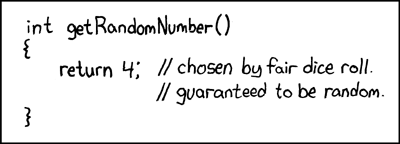
\includegraphics[scale=0.6]{xkcd/random_number} \\
%			%\vspace{-7pt}
%			{\url{http://xkcd.com/221}}
%		\end{figure}
%	}
%\end{frame}

\section{MIMA}

\begin{frame}{MIMA}
	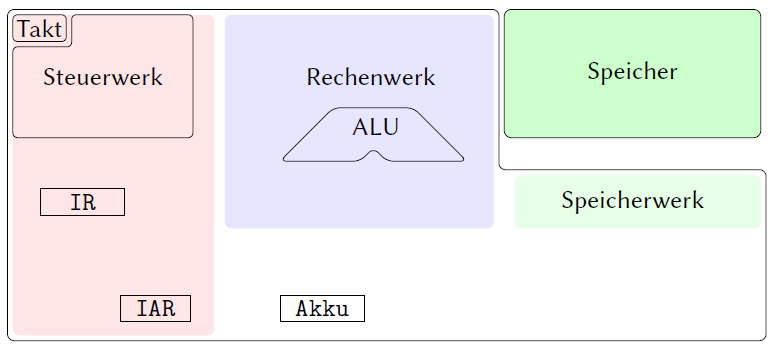
\includegraphics[width=\linewidth]{MIMA_simple.png}\\
	Die \emph{MIMA} ist ein idealisierter Prozessor. 
\end{frame}

\begin{frame}{Eigenschaften}
	\begin{itemize}[<+->]
		\item Adressen sind 20 Bit lang
		\item \enquote{Werte} sind 24 Bit lang
		\item Befehlscodierungen -- zwei Formate:
		\begin{itemize}
			\item[a)] 4 Bit für den OpCode und 20 Bit für einen Parameter (Adresse / Konstante)
			\item[b)] 8 Bit Befehl (Rest irrelevant)\\
			\item[]<+(-2)-> \includegraphics[width=100px]{MIMA_commands.png} 
		\end{itemize} 
	\end{itemize}
\end{frame}


\begin{frame}{Wichtige Register}
	\begin{itemize}[<+->]
		\item \emph{IAR} : InstruktionsAdressRegister : Speichert Adresse des aktuell auszuführenden Befehls.
		\item \emph{IR}: InstruktionsRegister : Speichert den auszuführenden Befehl selbst.
		\item \emph{SAR}: SpeicherAdressRegister : Enthält die Adresse eines Wertes, der aus dem Speicher gelesen werden soll.
		\item \emph{SDR}: SpeicherDatenRegister : Enthält einen Wert, der aus dem Speicher geladen wurde.
		\item \emph{Akku}: enthält Ausgangswerte/Ergebnisse von Berechnungen
	\end{itemize}
\end{frame}

\begin{frame}[t]{Aufbau}
	\begin{figure}
		\centering
		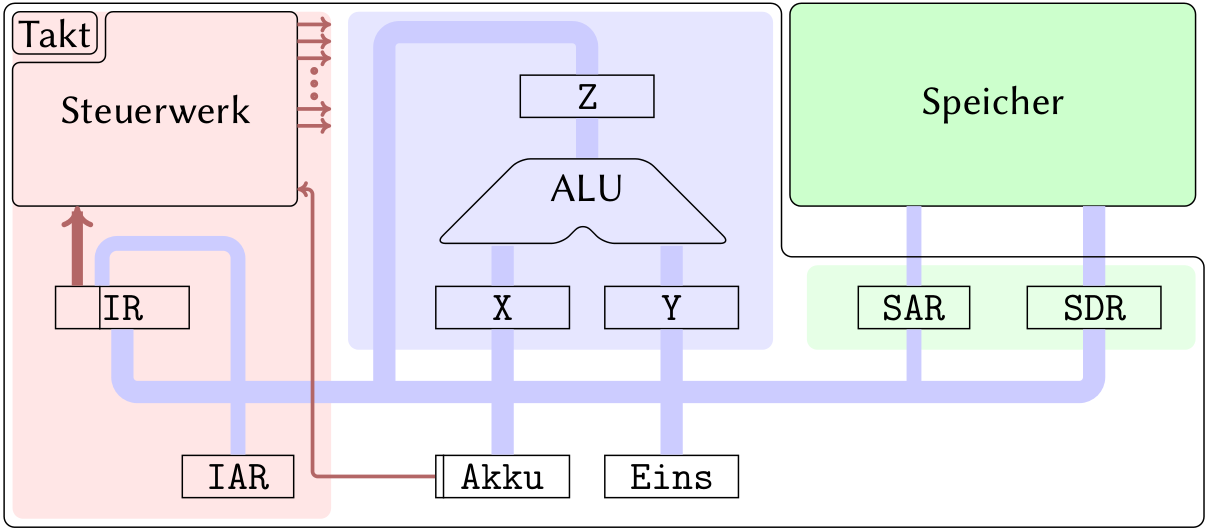
\includegraphics[width=\linewidth]{MIMA.png}
	\end{figure}
\end{frame}

\begin{frame}[t]{Befehlsholphase}
	\begin{figure}
		\centering
		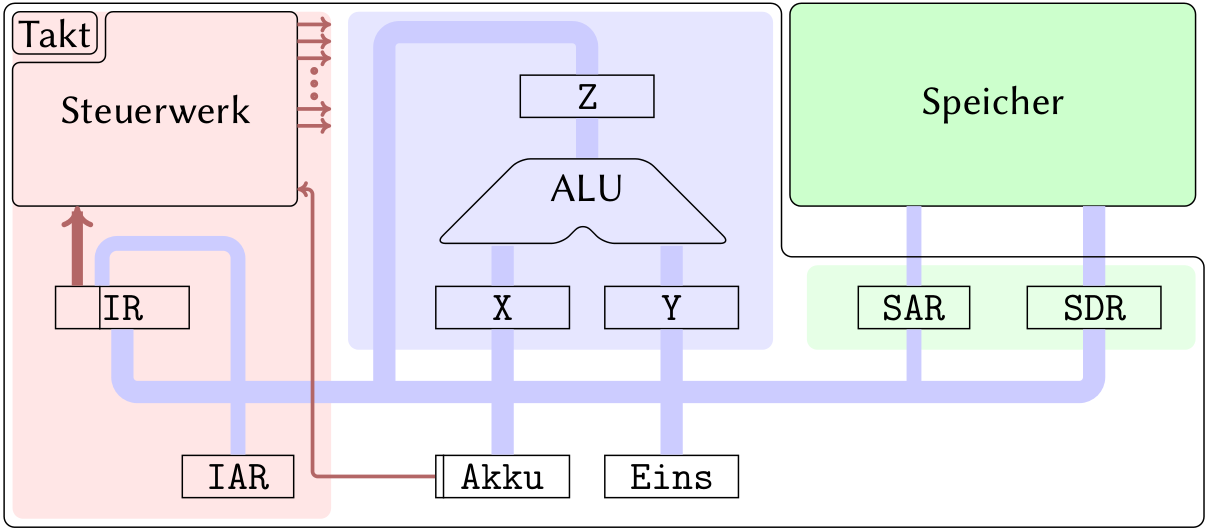
\includegraphics[width=\linewidth]{MIMA.png}
	\end{figure}
	\pause
	\only<2-6>{\begin{itemize}
		\only<2|handout:1> {\item[1.] IAR $\to $ SAR  und IAR $\to$ X 
			\item[] Befehlsadresse dem Speicher übergeben und Zähler zum Erhöhen an ALU geben.}
		\only<3|handout:2>{\item[2.] Eins $\to$ Y  
			\item[] 1-Wert für Erhöhung des Zählers an ALU geben.}
		\only<4|handout:3>{\item[3.] ALU aufaddieren ($Z=X+Y$) 
			\item[] Nächste Befehlsadresse berechnen. }
		\only<5|handout:4>{\item[4.] Z $\to$ IAR 
			\item[] Adresse für nächste Runde speichern. }
		\only<6|handout:5>{\item[5.] SDR $\to$ IR 
			\item[] Wert zur angefragten Adresse erhalten. }
	\end{itemize}}	
\end{frame}

\newcommand{\itemizeconfig}{\setlength{\parsep}{0pt}\setlength{\parskip}{0pt}\setlength{\topsep}{0pt}\setlength{\partopsep}{0pt}}
\newcommand{\explain}[1]{\hfill {\small #1 }}
\begin{frame}{Befehle}
	Die MIMA besitzt einen Befehlssatz mit möglichen Befehlen. %Andere Befehle (oder Varianten) werden NICHT unterstützt und können daher nicht verwendet werden!
	\textbf{Nur die Befehle aus der VL} dürft ihr benutzen! \\ 
	\smallskip
	(Befehle, die eigentlich zwei Operanden brauchen, lesen zusätzl. vom Akku.)
	{
	\begin{itemize}[<+->] \itemizeconfig
		\item Rechenoperationen:
		\begin{itemize} 
			\item ADD adr \explain{Akku $\leftarrow$ Akku + mem(adr)}
			\item AND, OR, XOR adr \explain{Dasselbe mit bitweisem Und, Oder und eXclusive OR}
			\item NOT, RAR \explain{Akku $\leftarrow$ not(Akku); \quad  Rotate-Akku-Right();}
		\end{itemize}
		\item Datentransport:
		\begin{itemize}
			\item LDC const \explain{Akku $\leftarrow$ const\quad (const ist dabei eine \textbf{20-Bit}-Konstante) }
			\item LDV, STV adr \explain{(Lese/Schreibe in/vom Akku von/an Adresse)}
			\item LDIV, STIV adr \explain{(Lese/Schreibe von/an Adresse, die an der Adresse steht)}
		\end{itemize}
		\item Vergleichsoperation: EQL adr \explain{(liefert $-1$ wenn Akku $=$ mem(adr), 0 sonst)}
		\item Sprünge:
		\begin{itemize}
			\item JMP adr \explain{Springe zu Befehl in Adresse adr}
			\item JMN adr \explain{Springe, falls Akku negativ \quad „JuMp if Negative“}
		\end{itemize}
		\item HALT \explain{Stoppt die MIMA}
	\end{itemize}}
\end{frame}

\begin{frame}{Bemerkungen}
	\begin{block}{Indirekte Adressierung (LDIV, STIV)}
		\centering
		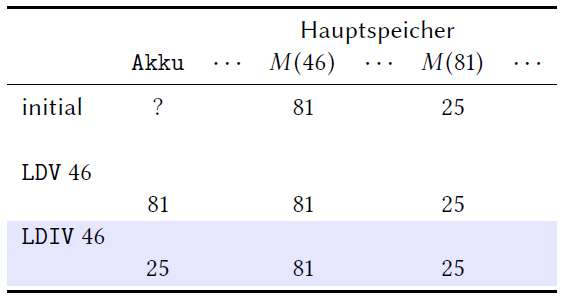
\includegraphics[width=150px]{MIMA_indirect.png}
	\end{block}
	
	\pause
	\begin{block}{HALT}
		Jedes Programm muss mit HALT enden! Sonst läuft das Programm endlos weiter! (Kostet dann Punkte!)
	\end{block}

	\pause
	\begin{block}{Negative Konstanten}
		Negative Konstanten können \textbf{nicht} mit LDC geladen werden. Warum? \\
		\pause \impl Unser Akku ist 24 Bit breit, aber wir können nur in die \textbf{hinteren 20 Bit} laden!
	\end{block}
\end{frame}

\begin{frame}{Negative Zahlen}
	\begin{block}{Aufgabe}
		An Adresse $a_1$ sei eine beliebige Zahl $x$ gegeben. Schreibt ein Programm, welches $-x$ (als Zweierkomplement) berechnet und an Adresse $a_2$ ablegt.
	\end{block}

	\visible<2|handout:2>{
		\begin{block}{Lösung}
			LDV $a_1$\\
			NOT\\
			STV $a_2$\\
			LDC 1\\
			ADD $a_2$\\
			STV $a_2$ \\
			HALT
		\end{block}
	}
\end{frame}

\begin{frame}{Beispiele}
	Beispiele zur Umsetzung von Anweisungen aus Hochsprachen (if, while, for....):\\
	\bigskip
	Siehe Übung Nr.~6 (WS 2018/19)
\end{frame}

\begin{frame}{Übung: Modulo 2 und Betrag}
	1. Schreibe ein Programm, das eine an Speicheradresse $a_1$ gegebenen positive Zahl Modulo 2 rechnet und an Adresse $a_2$ ablegt. \\
	\medskip
	2. Schreibe ein Programm, das den Betrag einer an Adresse $a_1$ gegebenen Zahl berechnet und an Adresse $a_2$ ablegt.
\end{frame}

\begin{frame}{Lösung: Modulo 2}
	\begin{tabbing}
		start: \; \= LDC 1 \quad  //$= 000000000000000000000001_2$ \\
				\> AND $a_1$ \\
				\> STV $a_2$ \\
				\> HALT
	\end{tabbing}
\end{frame}

\begin{frame}{Lösung: Betrag}
	\begin{tabbing}
		start: \quad \= LDV $a_1$ \\
					 \> JMN negate \\
		end: 		 \> STV $a_2$ \\
					 \> HALT \\
		negate:		 \> NOT \\
					 \> STV $a_2$ \\
					 \> LDC 1 \\
					 \> ADD $a_2$  \\
					 \> JMP end	 \\		 
	\end{tabbing}
\end{frame}

\begin{frame}{Übung: Modulo 3}
	Schreibe ein Programm, das eine an Speicheradresse $a_1$ gegebenen positive Zahl Modulo \textbf{3} (drei!) rechnet und an Adresse $a_2$ ablegt.
\end{frame}

\begin{frame}{Lösung: Modulo 3}
  \begin{tabbing}
    start: \quad \= LDC 1 \\
           \> STV One\\
           \> LDC 3\\
           \> NOT\\
           \> ADD One\\
           \> STV MinusThree\\
           \> LDV $a_1$\\
    \medskip
    while: \> ADD MinusThree\\
           \> JMN end\\
           \> JMP while\\
    \medskip
    end:   \> STV $a_1$\\
           \> LDC 3\\
           \> ADD $a_1$\\
           \> STV $a_2$ \\
           \> HALT\\
  \end{tabbing}
\end{frame}

%\begin{frame}{Noch offen: Klammerausdrücke}
%	A long, long time ago, in a land far away:\\
%	\medskip
%	Formale Sprachen angeben durch $\set{}, \*, {}^+, {}^*$...\\
%	Was ist mit der \textbf{Sprache aller gültigen Klammerausdrücke}? Können wir die auch so angeben?\\[1em]
%	\pause
%	\impl Jetzt wissen wir: \textbf{Nein}, das geht nicht! (Siehe VL)\\[1em]
%	
%	\begin{figure}[H]
%		\centering
%		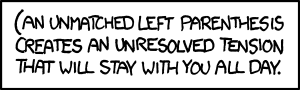
\includegraphics[scale=0.7]{xkcd/(.png}
%		\vspace{-7pt}
%		\caption{ \texttt{\url{https://xkcd.com/859/}} }
%	\end{figure}
%\end{frame}

\begin{frame}	
	\begin{block}{Was ihr nun wissen solltet}
		\begin{itemize}
			%\item Mehr Eigenschaften von Relationen
			\item Was die MIMA ist
			\item Wie man Programme in der MIMA schreibt
			%\item Wie man Sprachen mit Grammatiken beschreiben kann
			%\item Welche Eigenschaften Relationen haben können
		\end{itemize}
	\end{block}
	
	\begin{block}{Was nächstes Mal kommt}
		\begin{itemize}
			\item was kontextfreie Grammatiken sind
			\item Wie man Sprachen mit Grammatiken beschreiben kann
			\item Mehr Eigenschaften von Relationen
			%\item Nachts sind alle Katzen grau -- Prädikatenlogik
			%\item Algorithmen: Kochrezepte der Informatik
		\end{itemize}
	\end{block}
\end{frame}	

\xkcdframe{327}{Danke für eure Aufmerksamkeit! \smiley}{2.5}

\slideThanks

\end{document}